\documentclass[a4paper,12pt]{refrep}
\input{xcsoar.sty}

\title{Developer Manual}

\input{xcsoar-headers.sty}
\xcsoarheader{XCSoar Developer Manual}

\input{title-xcsoar.sty}
\usepackage{listings}

\usepackage{tikz}
\usetikzlibrary{arrows,shapes,fit,decorations,decorations.pathmorphing,decorations.pathreplacing,calc}

\tikzstyle{thread}=[draw, fill=lightgray, text centered,
  minimum width=7em, minimum height=2.5em]

\begin{document}
\maketitle

\input{toc.tex}

%%%%%%%%%%%%%%%%%%%%%%

\chapter*{Preface}

This manual applies to XCSoar version 7.0.  The authors reserve the
right to update this manual as enhancements are made throughout the
life of this product.

\section*{Warnings and precautions}

\warning IT IS THE USER'S RESPONSIBILITY TO USE THIS SOFTWARE PRUDENTLY. THIS
SOFTWARE IS INTENDED TO BE USED ONLY AS A NAVIGATION AID AND MUST NOT
BE USED FOR ANY PURPOSE REQUIRING PRECISE MEASUREMENT OF DIRECTION,
DISTANCE, LOCATION, OR TOPOGRAPHY. THIS SOFTWARE SHOULD NOT BE USED AS
AN AID TO DETERMINE GROUND PROXIMITY FOR AIRCRAFT NAVIGATION.
THIS SOFTWARE SHOULD NOT BE USED AS A TRAFFIC COLLISION AVOIDANCE SYSTEM.


\section*{Legal notices}

\subsection*{Software license agreement}

This software is released according to the GNU General Public License
Version~2.  See Appendix~\ref{cha:gnu-general-public} for the full
text of the agreement and warranty notice.

\subsection*{Limited liability}

In no event shall XCSoar, or its principals, shareholders, officers,
employees, affiliates, contractors, subsidiaries, or parent
organizations, be liable for any incidental, consequential, or
punitive damages whatsoever relating to the use of the Product.

\subsection*{Disclaimer}

This product, and all accompanying files, data and materials, are
distributed ``as is'' and with no warranties of any kind, whether
express or implied.  This product is used entirely at the risk of the
user.  Although great care has been taken to eliminate defects during
its development it is not claimed to be fault-free. No claims are made
regarding its correctness, reliability or fitness for any particular
purpose.  The XCSoar project developers and contributors shall not be
liable for errors contained herein or for incidental or consequential
damages, loss of data or personal injury in connection with
furnishing, performance, or use of this material.

%%%%%%%%%%%%%%%%%%%%%%%%%%%%%%%%%%%%%%%%%%%%%%%%%%%%%%%%%%%%%%%%

\chapter{Architecture}

This chapter describes XCSoar's internal code architecture.

\section{Source Organisation}

XCSoar's source code is stored in the \texttt{src} directory.  This
section tries to give a rough overview where you can find what.

\begin{itemize}

\item \texttt{Util/}: generic C++ utilities that do not depend on
  external libraries, such as data structures, string operations

\item \texttt{Math/}: math data types (fixed-point math, angles) and
  generic formulas

\item \texttt{Geo/}: geographic data structures and formulas

\item \texttt{Formatter/}: code that formats internal values to
  strings

\item \texttt{Units/}: conversion from SI units (``System'' units) to
  configured user units

\item \texttt{NMEA/}: data structures for values parsed from NMEA

\item \texttt{Profile/}: user profiles, loading from and saving to

\item \texttt{IGC/}: support for the IGC file format

\item \texttt{Logger/}: all loggers (NMEA, IGC, flights)

\item \texttt{Thread/}: multi-threading support (OS specific)

\item \texttt{Screen/}: base library for the graphical user interface

\item \texttt{Renderer/}: various graphical renderers, for map and
  analysis

\item \texttt{MapWindow/}: the map

\item \texttt{Form/}: modal dialogs and their controls (based on the
  screen library)

\item \texttt{Dialogs/}: modal dialogs implementations (based on the
  form library)

\item \texttt{Net/}: networking code (OS specific)

\item \texttt{Operation/}: generic code to support cancellable
  long-running operations

\item \texttt{Android/}: code specific to Android (the native part
  only; Java code is in \texttt{android/src/}

\item \texttt{Engine/PathSolvers/}: an implementation of Dijkstra's
  path finding algorithm, for task and contest optimisation

\item \texttt{Engine/Airspace/}: airspace data structures and airspace
  warnings

\item \texttt{Engine/Waypoint/}: waypoint data structures

\item \texttt{Engine/GlideSolvers/}: a MacCready implementation

\item \texttt{Engine/Task/}: task data structures and calculations

\item \texttt{Engine/Contest/}: contest optimisation

\item \texttt{Engine/Route/}: the route planner (airspace and terrain)

\end{itemize}

\section{Threads and Locking}

\subsection{Threads}

XCSoar runs on multiple threads, to make the UI responsive but still
allow expensive background calculations.

This is how it looks like on Windows and Linux/SDL (software
rendering):

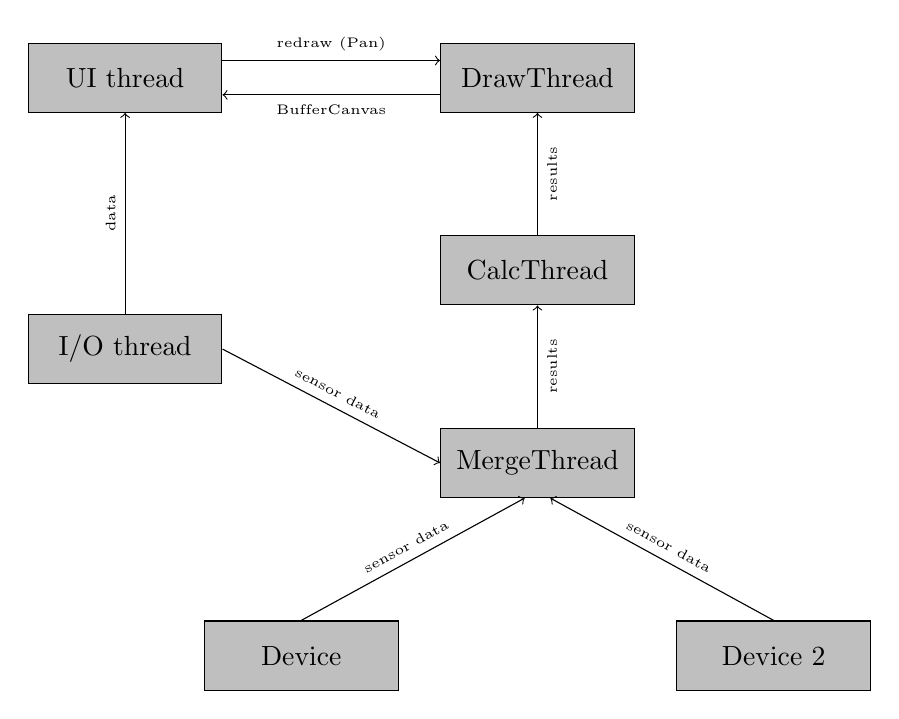
\begin{tikzpicture}
  \node(ui)[thread]{UI thread};

  \path(ui.east)+(4,0) node(draw)[thread]{DrawThread};
  \draw[->] (ui.10) -- (draw.170)
  node[midway, above, sloped, font=\tiny]{redraw (Pan)};
  \draw[->] (draw.190) -- (ui.350)
  node[midway, below, sloped, font=\tiny]{BufferCanvas};

  \path(draw.south)+(0,-2) node(calc)[thread]{CalcThread};
  \draw[->] (calc.north) -- (draw.south)
  node[midway, below, sloped, font=\tiny]{results};

  \path(calc.south)+(0,-2) node(merge)[thread]{MergeThread};
  \draw[->] (merge.north) -- (calc.south)
  node[midway, below, sloped, font=\tiny]{results};

  \path(merge.south)+(-3,-2) node(device1)[thread]{Device};
  \draw[->] (device1.north) -- (merge.250)
  node[midway, above, sloped, font=\tiny]{sensor data};

  \path(merge.south)+(3,-2) node(device2)[thread]{Device 2};
  \draw[->] (device2.north) -- (merge.290)
  node[midway, above, sloped, font=\tiny]{sensor data};

  \path(ui.south)+(0,-3) node(io)[thread]{I/O thread};
  \draw[->] (io.north) -- (ui.south)
  node[midway, above, sloped, font=\tiny]{data};
  \draw[->] (io.east) -- (merge.west)
  node[midway, above, sloped, font=\tiny]{sensor data};
\end{tikzpicture}

The UI thread is the main thread.  It starts the other threads and is
responsible for the UI event loop.  No other thread is allowed to
manipulate windows.  The UI thread has a timer which does regular
house keeping twice per second (\texttt{Pro\-cess\-Ti\-mer.cpp}).

The calculation thread (\texttt{Calcu\-la\-tion\-Thread.cpp},
\texttt{Glide\-Com\-pu\-ter*.cpp}) does all the expensive calculations
in background.  It gets data from the devices (through
\texttt{Merge\-Thread}) and forwards it together with calculation
results to the drawing thread and the main thread.

Each device has its own thread (\texttt{Serial\-Port.cpp}).  This is
needed because Windows CE does not support asynchronous COMM port I/O.
The thread is stopped during task declaration (which happens in the UI
thread).

When new data arrives on the serial port, the \texttt{Merge\-Thread}
gets notified, which will merge all sensor values into one data
structure.  It will then run cheap calculations, and forwards
everything to the \texttt{Calcu\-la\-tion\-Thread}.

With OpenGL, the map is rendered live without a buffer.  There is no
DrawThread.

On Android, the UI thread is not the main thread - the main thread is
implemented in Java, managed by Android itself.  The UI thread listens
for events which the Java part drops into the event queue
(\texttt{NativeView.java} and others).  The internal GPS does not need
a thread, it is implemented with Java callbacks.  For Bluetooth I/O,
there are two threads implemented in Java (\texttt{InputThread.java}
and \texttt{OutputThread.java}, managed by
\texttt{BluetoothHelper.java}).

\subsection{Locking}

Some data structures are rarely modified.  There is no lock for them.
For a modifications, all threads must be suspended.  Example:
waypoints, airspaces.

Other data structures are modified so often that correct locking would
be too much overhead.  Each thread and each instance has its own
copy.  The lock needs to be obtained only for making the private
copy.  The private copy can be used without locking.  Example:
\texttt{NMEA\_INFO}, \texttt{DERIVED\_INFO}.

There are objects which are too expensive to copy.  Normal locking
applies to them.  We have a template class called \texttt{Guard} to
enforce proper read/write locking.  Example: the task.


\section{Accessing Sensor Data}

Much of XCSoar deals with obtaining sensor data and visualising it.

Suppose you want to write a dialog that needs the current GPS
location, where do you get it?  The short and simple answer is: from
\verb|CommonInterface::Basic()| (the \texttt{InterfaceBlackboard}).
Example:

\begin{verbatim}
#include "Interface.hpp"

...
  const auto &basic = CommonInterface::Basic();
  if (basic.location_available)
    current_location = basic.location;
\end{verbatim}

This is true for the main thread (aka the ``user interface thread'').
Other threads must not use the \texttt{Interface.hpp} library, because
the \verb|InterfaceBlackboard| is not protected in any way.  It
contains copies of various data structures just for the main thread.

This is how sensor data moves inside XCSoar:

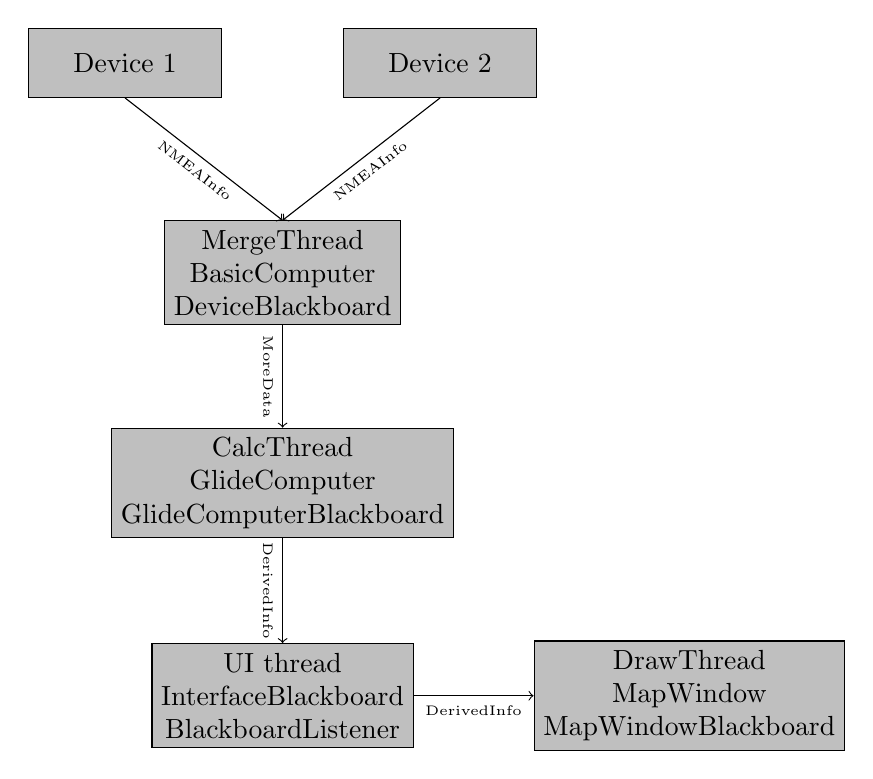
\begin{tikzpicture}
  \node(merge)[thread,align=center]{
    MergeThread\\
    BasicComputer\\
    DeviceBlackboard
  };

  \path(merge.north)+(-2,2) node(device1)[thread]{Device 1};
  \draw[->] (device1.south) -- (merge.north)
  node[midway, below, sloped, font=\tiny]{NMEAInfo};

  \path(merge.north)+(2,2) node(device2)[thread]{Device 2};
  \draw[->] (device2.south) -- (merge.north)
  node[midway, below, sloped, font=\tiny]{NMEAInfo};

  \path(merge.south)+(0,-2) node(calc)[thread,align=center]{
    CalcThread\\
    GlideComputer\\
    GlideComputerBlackboard
  };
  \draw[->] (merge.south) -- (calc.north)
  node[midway, below, sloped, font=\tiny]{MoreData};

  \path(calc.south)+(0,-2) node(ui)[thread,align=center]{
    UI thread\\
    InterfaceBlackboard\\
    BlackboardListener
  };
  \draw[->] (calc.south) -- (ui.north)
  node[midway, below, sloped, font=\tiny]{DerivedInfo};

  \path(ui.east)+(3.5,0) node(draw)[thread,align=center]{
    DrawThread\\
    MapWindow\\
    MapWindowBlackboard
  };
  \draw[->] (ui.east) -- (draw.west)
  node[midway, below, sloped, font=\tiny]{DerivedInfo};
\end{tikzpicture}

The device driver parses input received from its device into its own
\texttt{NMEAInfo} instance inside \texttt{DeviceBlackboard}
(i.e. \verb|per_device_data|).  Then it wakes up the
\texttt{MergeThread} to merge the new data into the central
\texttt{NMEAInfo} instance.  The \texttt{MergeThread} hosts the
\texttt{BasicComputer} which attempts to calculate missing data (for
example, derives vario from GPS altitude).

The \texttt{CalculationThread} wakes up and receives the
\texttt{MoreData} object from \texttt{DeviceBlackboard}.  Here,
expensive calculations are performed (\texttt{GlideComputer}: task
engine, airspace warnings, ...), resulting in a \texttt{DerivedInfo}
object.  The \texttt{CalculationThread} runs no more than twice per
second.

Finally, the UI thread wakes up and receives \texttt{MoreData} and
\texttt{DerivedInfo} via \texttt{DeviceBlackboard}.  This updates
InfoBoxes and other UI elements.  On Windows, the map is drawn in a
separate thread, so there's another layer.

Let's get back to the question: where do I get sensor data?  That
depends on who you are:

\begin{itemize}

\item you are the user interface: (InfoBoxes, dialogs, any Window
  callback): \texttt{InterfaceBlackboard} (see above).  To get
  notified on changes, register a \texttt{BlackboardListener} (and
  don't forget to unregister it).

\item you are the MapWindow: depends!  If you're being called from
  \texttt{OnPaintBuffer} (i.e.\ inside the \texttt{DrawThread}), you
  must use the \texttt{MapWindowBlackboard}, all others must use the
  \texttt{InterfaceBlackboard}.

\item you are a ``computer'' library: you will get the values as a
  parameter.  Don't try to use the \texttt{GlideComputerBlackboard}
  directly.

\item you are a device driver: implement the method
  \texttt{OnSensorUpdate} or \texttt{OnCalculatedUpdate} if you need
  to know values from other devices or calculation results.

\item everybody else may use the \texttt{DeviceBlackboard}, but be
  sure to lock it while using its data.

\end{itemize}


\chapter{Developing}

\section{Debugging XCSoar}

The XCSoar source repository contains a module for the GNU debugger
(\texttt{gdb}).  It contains pretty-printers for various XCSoar types,
including \texttt{Angle}, \texttt{GeoPoint} and others.  These are
helpful when you print values in the debugger.  To use it, start the
debugging session and load the module:

\begin{verbatim}
$ gdb -ex "source tools/gdb.py" output/UNIX/bin/xcsoar
(gdb) run
\end{verbatim}

The module will automatically convert fixed-point to floating point,
radian angles to degrees and more.  You can now do fancy stuff like:

\begin{verbatim}
(gdb) p basic.location
$1 = GeoPoint(7.93911242887 51.1470221074)
(gdb) p basic.date_time_utc
$2 = DateTime(2012/12/23 21:41:57)
(gdb) p basic.track
$3 = 55.2254197961
(gdb) p basic.external_wind
$4 = GeoVector::ZERO
(gdb) p current_leg.vector_remaining
$5 = GeoVector(267.899420345 107957.109724)
\end{verbatim}



%%%%%%%%%%%%%%%%%%%%%%%%%%%%%%%%%%%%%%%%%%%%%%%%%%%%%%%%%%%%%%%
\chapter{User interface guidelines}

\section{General}

\begin{itemize}
\item Minimise the number of colours, and re-use colour groups already defined.
\item Too much use of colour where it is not required serves only to reduce 
 the effectiveness of bright colours for important items.
\item High colour saturation elements should be reserved for high importance items
\item High contrast against background should be reserved for high importance items
\item Attempt to adopt colours that are intuitive based the function of the item
\item Minimise the clutter where possible --- readibility is essential for use 
 in flight
\item Use colours defined in \verb|Graphics| according to functional name, not 
 their actual colour.
\item Try to maintain consistent use of colours in all uses of that function, 
 such as dialogue graphics as well as map overlays and infoboxes.
\item Text should always be monochrome.
\end{itemize}

Use aviation conventions or adopt best aviation human factors
standards where possible, in particular:
\begin{itemize}
\item ICAO Internation Standards and Recommended Practices, Annex 4 to the 
 Convention on International Civil Aviation (Aeronautical Charts).
\item NASA Colour Usage recommendations and design guidelines: \verb|http://colorusage.arc.nasa.gov/|
\item DOT/FAA/AR-03/67 {\em Human Factors Considerations in the Design and 
 Evaluation of Electronic Flight Bags (EFBs)} \verb|http://www.volpe.dot.gov/hf/aviation/efb/docs/efb_version2.pdf|
\item FAA Human Factors Design Standards \verb|http://hf.tc.faa.gov/hfds/|.
\item DOT/FAA/AM-01/17 {\em Human Factors Design Guidelines for Multifunction Displays}
\end{itemize}

Check for performance with respect to colour blindness.
This site has a useful tool that can be used to convert screenshots
to how they would look to a person with common color blindness:
\verb|http://www.etre.com/tools/colourcheck/|.

{\bf For safety purposes, avoid use of elements that may encourage or require 
the user to stare at the screen continuously.}

{\bf For safety purposes, avoid user controls that have significant risk of 
producing unsafe results if misconfigured by the pilot.}

\subsection{General colour conventions}
Colour conventions generally in use throughout the program:
\begin{itemize}
\item Red for indicator of warning
\item Orange for indicator of caution
\item Green for positive indicator of safety
\item Blue for neutral indicator of safety
\end{itemize}

\subsection{Displayed data}
\begin{itemize}
\item Where data is invalid, indicate this by not presenting the data or
  showing dashes.
\item Present data in user-defined units.
\item Display numerical data with significant digits appropriate to the accuracy of the
  calculations, or its functional use by the pilot, whichever is lower.
\end{itemize}

\section{Dialogs and menu buttons}

\subsection{Colors}
Colour conventions in use are:
\begin{itemize}
\item Grey for buttons
\item Buttons and other widgets rendered with an evenly shaded border
\item Yellow for clicked items
\item Light blue for the key focused item
\item Medium blue for dialogue title bar
\item Text is black if the item is enabled
\item Text is greyed out (but still visible) if the item is disabled
\end{itemize}

\subsection{dialogue types and navigation buttons}
There are four types of dialogs in XCSoar, and the navigation 
buttons for each are different.  
Navigation buttons are the Close, OK, Cancel and Select buttons.
\begin{itemize}
\item Dialogs that modify and save data when the dialogue closes.

These shall usually have a Close button (no Cancel) and may have context specific 
function buttons
\item Dialogs that modify data where Cancel would be important for the user.

These shall have OK and Cancel buttons.  This may include dialogs with 
children dialogs where hitting Cancel from the parent dialogue cancels 
all the changes made in the children dialogs

\item Dialogs that have a list of values, one of which can be selected to 
 return to the parent dialogue.

These shall have Select and Cancel buttons
\item Dialogs that display information that cannot be modified.

These shall have a Close button
\end{itemize}

\subsection{dialogue button placement and size}
\begin{itemize}
\item The Close and Cancel buttons will never appear in the same dialogue and 
 are always located in the same place.  This location will be:

For portrait: lower right

For landscape: lower left
\item The Select button will be accompanied with a Cancel button.  The locations will be:

For portrait: Select in lower left, Cancel in lower right

For landscape: Cancel in lower left, Select immediately above it
\item Buttons will be 35 (scaled) pixels high
\item Buttons will be flush with the bottom of the screen and with the sides of 
 the screen and against each other (no margins)
\item In portrait, buttons will be 33% or 50% or 100% width of the screen
\item In landscape, buttons will be 65 to 80 (scaled) pixels wide, as wide as the 
 frame permits.  They will generally be a vertical row of buttons flush left of the screen
\item If text won't fit on a button, the buttons can be made larger consistently 
 for a screen, but this should be the exception because if it must contain that 
 much text consider using a different type of control.
\item Exceptions to all the dialogue concepts above are encouraged, but should be 
 mocked up and reviewed with the development community prior to implementing and 
 possibly documenting in the developers guide.
\end{itemize}

\subsection{Usability}
\begin{itemize}
\item Minimum size of buttons should be X by Y mm
\item Ensure all dialogs are navigable using cursor keys only
\item Ensure the focussed item is clearly identified.  The rectangle
  of the widget on the canvas may be drawn using the \verb|fill_focus| method
  of \verb|Canvas|.
\end{itemize}

\section{Main graphics}

\subsection{Colors}
Colour conventions in use, in order of priority, are:
\begin{itemize}
\item Aircraft black and white, for neutrality but clear identification
\item Traffic (FLARM) use alarm green, orange, and red.
\item Lift is vibrant green, sink is copper orange.
\item Aircraft navigation (route, best cruise track) is (ICAO) dark purple-blue
\item Task navigation lines and areas are (ICAO) magenta.
\item Updraft sources and other updraft derived data is sky blue.
\end{itemize}

(Todo) airspace alert colours

Map culture (topography) and terrain rendering should conform to ICAO
Annex 4 where appropriate.  Note that some modifications are
reasonable for electronic use given that Annex 4 deals with paper
charts.  Nevertheless, the colour conventions are useful to adopt as they are
likely to be intuitive and are designed for aviation use.

\subsection{Pen styles}

\begin{itemize}
\item Map culture should be rendered with a thin pen
\item Thicker pens used for important (e.g.\ task, navigational, airspace) lines
\item Dashed lines are used to increase perceptual priority
\end{itemize}

\subsection{Map overlays}
Elements on the map that are not part of the map layer, such as additional
informational widgets (final glide bar, wind, north arrow) should be rendered
so as to help those elements be visually separated from the map:

\begin{itemize}
\item Generally adopt higher contrast (higher colour saturation or darker shade) 
 than the background map layer elements.

\item For elements covering an area (non line), draw the entire element or a border
with a luminosity contrasting pen, of width \verb|IBLSCALE(1)|.

\item Consider whether the widget is required in all flying states and display modes.
if it does not serve a direct functional purpose in some states/modes, do not
render it.

\item Avoid locating widgets at the aircraft symbol (ownship symbol).
It is important to keep this area clear so the aircraft symbol can be easily found.

\end{itemize}

Elements that may be rendered over each other should be organised in order of
priority, particularly with alert warning items above caution items above non-alert items.

\section{Terminology}
\subsection{Glide Ratio}
'Glide ratio' is a non-specific term which can refer to the ratio of horizontal to 
vertical motion with reference to either the surrounding airmass or the ground.

To reduce confusion, ground-referenced glide ratios (eg distance travelled over 
ground vs altitude lost) should be referred to by the term 'glide ratio over 
ground' when space allows, or 'glide ratio' / 'GR'.

Air-referenced glide ratios (eg airspeed vs sink rate) should be specified as 
'lift/drag ratio' / 'L/D ratio' / 'LD'. The lift/drag ratio is numerically equal 
to the air-referenced glide ratio when flying at constant speed.

If usage spans both air-referenced and ground-referenced glide ratios, the 
non-specific term 'glide ratio' / 'GR' should be used. 'Lift/drag ratio' should 
never be used to refer to ground-referenced glide ratios.

\chapter{File formats}\label{cha:file_formats}

\input{tpl_format.tex}


%%%%%%%%%%%%%%%%%%%%%%%%%%%%%%%%%%%%%%%%%%%%%%%%%%%
\appendix

\chapter{Setting up a development environment based on linux}\label{cha:developmentsetup}
\input{developsetuplinux.tex}

\chapter{Building a KOBO Kernel}\label{cha:kobokernelbuild}
This is step-by-step instructions on how to cross compile a Kobo kernel to modify the
kernel, add modules or both.  This is needed for OTG support.

Although most, if not all, Kobo hardware supports OTG, most models have OTG disabled
in the kernel.  Even the one model (as of Jan 2022) that has it enabled is missing many
modules.  By following this guide, OTG support can be added.  Note older Kobos use 
uImage but newer ones use zImage.

The following has been tested for only one model of Kobo (ClaraHD) and only one XCSoar
development environment (Debian 11 with sudo, git and the two ide/provisioning scripts
run).

\section{Install additional tools on development machine}
Login to the development machine and install tools as follows:

\begin{verbatim}
sudo apt-get install bc
sudo apt-get install lzop
\end{verbatim}

\section{Get kernel information}
On the relevant model of Kobo, make sure it is updated and loaded with XCSoar.  Boot
the Kobo and at the splash screen choose Network then connect to WiFi and enable Telnet.
Get the IP address from the Wifi menu then connect to the Kobo with telnet using PuTTY
or similar terminal program.  From there get the data as follows:

\begin{verbatim}
cat /proc/version
\end{verbatim}

The text returned contains both the kernel version and the gcc version.
For everything that follows, use only the kernel version triplet such as 4.1.15
and ignore anything after the ``-``.  For the gcc version use the triplet such as 5.3.0.

Next get the kernel config file as follows:

\begin{verbatim}
zcat /proc/config.gz >/mnt/onboard/config
\end{verbatim}

Download the /mnt/onboard/config file to your home directory.

\section{Install toolchain for arm-linux-gnueabihf}
To compile the kernel you must install a toolchain (gcc, g++ etc.) of the version with
which the kernel was compiled (as determined above).  There are many toolchains available
and you can either install a binary or compile one.  An example using linaro follows:

\begin{verbatim}
go to 
  https://releases.linaro.org/components/toolchain/binaries
select the most recently dated folder for the 
  compiler version determined above (e.g. 5.3-2016.05)
select the platform as arm-linux-gnueabihf
download the tar.xz file for x86_64_arm_linux_gnueabihf to /opt
  Note the third number of the version may differ
  (e.g. 5.3.1 instead of 5.3.0)
cd /opt
sudo tar -xvf <filename>
\end{verbatim}

Do not add the toolchain to the path but note the directory that contains the binaries such as
gcc and g++.  Also, make note of the prefix on the binaries (such as arm-linux-gnueabihf-).

\section{Install kernel source}
Slightly outdated but suitable sources for the kernels for the different models are kept
on GitHub in the Kobolabs/Kobo-Reader repository.  Note it is filed by chipset though the
model may also be shown.  If needed, to find the right chipset google for the Kobo wiki.

Download the appropriate .bz2 file to your home directory then enter the following commands:

\begin{verbatim}
cd
sudo tar -xvf <filename>
cd kernel
sudo make CROSS_COMPILE=<binary path>/<binary prefix> \
  ARCH=arm distclean
\end{verbatim}

Add the config file to the source and update it.

\begin{verbatim}
cd
cp config ./kernel/.config
cd kernel
sudo make CROSS_COMPILE=<binary path>/<binary prefix> \
  ARCH=arm oldconfig
\end{verbatim}

\section{Build the kernel}
It is now ready to attempt to build the original kernel.
If there are errors, edits must be made to
successfully compile the kernel.

\begin{verbatim}
sudo make CROSS_COMPILE=<binary path>/<binary prefix> \
  ARCH=arm clean
sudo make CROSS_COMPILE=<binary path>/<binary prefix> \
  ARCH=arm vmlinux
\end{verbatim}

If you get an error "/usr/bin/ld: scripts/dtc/dtc-parser.tab.o:(.bss+0x50):
multiple definition of `yylloc'" it is because older toolchains default
to warn on duplicate definitions and newer ones fail.  Correct it as follows:

\begin{verbatim}
sudo nano scripts/dtc/dtc-parser.tab.c
  change
    YYLTYPE yylloc;
  to
    extern YYLTYPE yylloc;
sudo make CROSS_COMPILE=<binary path>/<binary prefix> \
  ARCH=arm vmlinux
\end{verbatim}

If you get an error "<filename><address> error: implicit declaration of function"
for function pinctrl\_pm\_select\_sleep\_state or
pinctrl\_pm\_select\_default\_state or pinctrl\_pm\_lookup\_state it is because
older toolchains default to warn on implicit declarations and newer ones fail. 
Correct it as follows:

\begin{verbatim}
sudo nano <filename>
  add
    #include <linux/pinctrl/consumer.h>
  to the bottom of the #include <linux...> list
sudo make CROSS_COMPILE=<binary path>/<binary prefix> \
  ARCH=arm vmlinux
\end{verbatim}

If you get an error about missing imx6sll-e80k02-base.dts the e60 file is the
same as the e80 file for our purposes so use it as follows:

\begin{verbatim}
cd arch/arm/boot/dts
ln -s imx6sll-e60k02-base.dts ims6sll-e80k02-base.dts
sudo make CROSS_COMPILE=<binary path>/<binary prefix> \
  ARCH=arm vmlinux
sudo make CROSS_COMPILE=<binary path>/<binary prefix> \
  ARCH=arm modules
sudo make CROSS_COMPILE=<binary path>/<binary prefix> \
  ARCH=arm zImage
\end{verbatim}

\section{Edit the kernel configuration and rebuild}
At this point you should have a successful build of factory kernel.  Now it is necessary
to edit the kernel as needed to support the desired OTG capabilities.  The main
functions and drivers which should be supported are OTG, sound, network and  serial.
Specifically for Clara HD, OTG was already enabled so this involved adding modules, not
built in functionality.  The changes were made as follows:

\begin{verbatim}
sudo make CROSS_COMPILE=<binary path>/<binary prefix> \
  ARCH=arm menuconfig
Go to Device Drivers | USB support
Change USB Serial Converter support to "M"
Go to USB Serial Converter support
Change AIRcable Bluetooth... to "M"
Change Winchiphead CH341... to "M"
Change CP210x family... to "M"
Change FTDI Single... to "M"
Change Garmin GPS Driver to "M"
Change Moschip 7840... to "M"
Change Navman GPS device... to "M"
Change Prolific 2303 Single... to "M"
Back out to Device Drivers
Go to Sound card support
Go to Advanced Linux Sound Architecture
Go to USB sound devices
Change USB Audio/MIDI driver to "M"
Back out to Device Drivers
Go to Network device support
Change USB Network Adapters to "M"
Go to USB Network Adapters
Change Multi-purpose USB Networking... to "M"
Change ASIX AX88xxx... to " "
Change ASIX AX88179... to " "
Change CDC EEM support to "M"
Change CDC NCM support (NEW) to "M"
Change NetChip 1080... to " "
Change Host for RNDIS... to "M"
Change Simple USB Network... to "M"
Change eTEK based... to " "
Change Embedded ARM... to " "
Change Sharp Zaurus... to " "
save as .config (default) then exit
sudo make CROSS_COMPILE=<binary path>/<binary prefix> \
  ARCH=arm vmlinux
sudo make CROSS_COMPILE=<binary path>/<binary prefix> \
  ARCH=arm zImage
sudo make CROSS_COMPILE=<binary path>/<binary prefix> \
  ARCH=arm modules
\end{verbatim}

\section{Create the file for the XCSoar build}

If you are building a new kernel (i.e. original kernel doesn't support OTG), the desired
file is created already as the zImage file and must be copied or moved to the
/opt/kobo/kernel folder on the XCSoar build machine.  If the factory kernel already
supports OTG, the desired file is a file of loadable modules for the factory kernel.
To create the file of loadable modules, proceed as follows for the example of Clara HD:

\begin{verbatim}
cd ~/kernel
sudo install -d -m 775 -g root -o root \
  modules
sudo install -d -m 775 -g root -o root \
  modules/<kernel version>
sudo install -d -m 775 -g root -o root \
  modules/<kernel version>/drivers
sudo install -d -m 775 -g root -o root \
  modules/<kernel version>/drivers/usb
sudo install -d -m 775 -g root -o root \
  modules/<kernel version>/drivers/usb/serial
sudo install -D -m 644 -g root -o root \
  drivers/usb/serial/*.ko \
  modules/<kernel version>/drivers/usb/serial
sudo install -d -m 775 -g root -o root \
  modules/<kernel version>/drivers/net
sudo install -d -m 775 -g root -o root \
  modules/<kernel version>/drivers/net/usb
sudo install -D -m 644 -g root -o root \
  drivers/net/*.ko \
  modules/<kernel version>/drivers/net
sudo install -D -m 644 -g root -o root \
  drivers/net/usb/*.ko \
  modules/<kernel version>/drivers/net/usb
sudo install -d -m 775 -g root -o root \
  modules/<kernel version>/sound
sudo install -d -m 775 -g root -o root \
  modules/<kernel version>/sound/usb
sudo install -D -m 644 -g root -o root \
  sound/usb/*.ko \
  modules/<kernel version>/sound/usb
sudo install -d -m 775 -g root -o root \
  modules/<kernel version>/sound/core
sudo install -D -m 644 -g root -o root \
  sound/core/*.ko \
  modules/<kernel version>/sound/core
tar -czvf ClaraHD_OTG_Drivers.tgz modules
sudo mkdir /opt/kobo
sudo mkdir /opt/kobo/kernel
sudo cp ClaraHD_OTG_Drivers.tgz /opt/kobo/kernel
\end{verbatim}


\chapter{GNU General Public License}\label{cha:gnu-general-public}
\input{gpl.tex}

\end{document}
